\section{Results}\label{sec:results}
All results are at a three-hour step with the weather years 2016--2019, unless stated. Costs are per MWh of the demand not met by existing hydropower. The saving is the cost of the least-cost system without any nuclear minus the cost of the system with nuclear. All numbers come from the runs, through the report generated from them (\texttt{docs/results\_v8.md} in the repository), which also lists the six-hour runs and the review checks.

\subsection{Central results}\label{sec:central}
Table~\ref{tab:central} gives the free optimum of the four central cases. At 5\% the least-cost system has 23.2\,GW of nuclear in PI and 15.7\,GW in OB, 44.5\% and 30.5\% of demand; nuclear lowers the system cost by 13.35 and 6.86\,EUR/MWh, that is EUR\,4.8 and 2.4 billion a year. At 7\% the optimum is 15.6\,GW in PI and 11.1\,GW in OB. The OB optimum at 7\% consists only of SMRs, whose target cost is then just below that of large reactors (Section~\ref{sec:smr}); with SMRs switched off it is 11.0\,GW of large reactors, at a cost of 131.43 against 131.16\,EUR/MWh. At 5\% no SMR is built and the OB optimum is the same with and without them.

\begin{table}[!tb]
\centering\footnotesize
\caption{Central results: free optimum at a three-hour step. Nuclear includes SMRs. Costs in EUR/MWh; share of total demand, exported nuclear energy included.}\label{tab:central}
\begin{tabular}{@{}llrrrrrrr@{}}
\toprule
Case & Rate & Nuclear & of which & Share of & Cost with & Cost without & Saving & Saving\\
 & & GW & SMR, GW & demand, \% & nuclear & nuclear & EUR/MWh & EUR billion/yr\\
\midrule
PI & 5\% & 23.2 & 0.0 & 44.5 & 114.42 & 127.77 & 13.35 & 4.8\\
PI & 7\% & 15.6 & 0.0 & 29.9 & 141.00 & 149.58 & 8.59 & 3.1\\
OB & 5\% & 15.7 & 0.0 & 30.5 & 107.53 & 114.39 & 6.86 & 2.4\\
OB & 7\% & 11.1 & 11.1 & 21.6 & 131.16 & 133.79 & 2.63 & 0.9\\
\bottomrule
\end{tabular}
\end{table}

\subsection{Value curves}\label{sec:curves}
Figure~\ref{fig:value} and Table~\ref{tab:value} give the marginal value of each 4\,GW block of nuclear capacity, from Eq.~\eqref{eq:value}; the system costs $C(N)$ behind them are in Appendix~\ref{app:curves}. The curves do not depend on the cost assumed for nuclear.

In PI at 5\% the first 4\,GW are worth 1{,}318\,EUR/kW-yr and the value falls to 921 for the block from 20 to 24\,GW and to 868 for the next one: the central cost of 911 lies between them, consistent with the free optimum of 23.2\,GW. In OB without SMRs the first 4\,GW are worth 1{,}145\,EUR/kW-yr, and the central cost lies between the blocks from 12 to 16\,GW (965) and from 16 to 20\,GW (877). At 7\% every block is worth more than at 5\%, because the alternatives also cost more, but the cost of nuclear rises more than its value: the central cost of 1{,}239 lies between the blocks from 12 to 16\,GW (1{,}286) and from 16 to 20\,GW (1{,}162) in PI, and between those from 8 to 12\,GW (1{,}262) and from 12 to 16\,GW (1{,}148) in OB without SMRs.

\begin{figure}[!tb]
\centering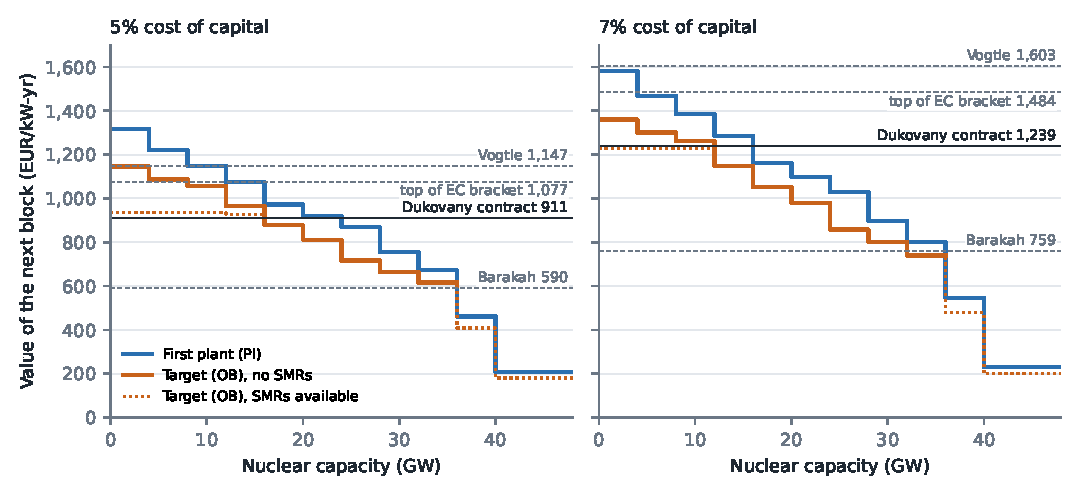
\includegraphics[width=0.84\linewidth]{fig_value_en.pdf}
\caption{Value curve of nuclear capacity: annual fixed cost at which each block of 4\,GW is worth building (8\,GW for the last block), at a 5\% and a 7\% real cost of capital, three-hour step. Horizontal lines: fixN of four cost cases (``Dukovany contract'' is the central case, ``EC bracket'' the Commission's bracket for the overnight cost). Dotted line: OB with SMRs available at target cost, where the fixed capacity is that of large reactors. Source: \texttt{results/v8\_runs.jsonl}.}\label{fig:value}
\end{figure}

\begin{table}[!tb]
\centering\footnotesize
\caption{Marginal value of nuclear capacity by block, EUR/kW-yr, three-hour step. The OB curves without SMRs were computed up to 36\,GW; the two OB curves coincide from 16\,GW at 5\% and from 12\,GW at 7\%.}\label{tab:value}
\begin{tabular}{@{}lrrrrrr@{}}
\toprule
 & \multicolumn{3}{c}{5\% (central fixN 911)} & \multicolumn{3}{c}{7\% (central fixN 1{,}239)}\\
\cmidrule(lr){2-4}\cmidrule(l){5-7}
Block, GW & PI & OB, no SMR & OB, SMR available & PI & OB, no SMR & OB, SMR available\\
\midrule
0--4 & 1{,}318 & 1{,}145 & 934 & 1{,}582 & 1{,}360 & 1{,}231\\
4--8 & 1{,}220 & 1{,}087 & 934 & 1{,}467 & 1{,}301 & 1{,}231\\
8--12 & 1{,}149 & 1{,}058 & 934 & 1{,}387 & 1{,}262 & 1{,}228\\
12--16 & 1{,}074 & 965 & 927 & 1{,}286 & 1{,}148 & 1{,}148\\
16--20 & 973 & 877 & 877 & 1{,}162 & 1{,}054 & 1{,}054\\
20--24 & 921 & 812 & 812 & 1{,}098 & 981 & 981\\
24--28 & 868 & 717 & 717 & 1{,}028 & 858 & 858\\
28--32 & 755 & 663 & 663 & 898 & 802 & 802\\
32--36 & 672 & 616 & 616 & 800 & 740 & 740\\
36--40 & 462 & & 409 & 545 & & 479\\
40--48 & 209 & & 180 & 230 & & 201\\
\bottomrule
\end{tabular}
\end{table}

\subsection{Cost cases read on the curves}\label{sec:casesres}
Table~\ref{tab:casesres} reads the eight cost cases of Table~\ref{tab:cases} on the 5\% curves, and two financing cases in which nuclear alone pays 6\% or 7\%; the 7\% curves and the OB curve with SMRs are in Appendix~\ref{app:curves}. In PI the best capacity on the grid is 24\,GW for the central case and for the 7-year build, 16\,GW for the risk median and for the midpoint of the Commission bracket (12 to 24\,GW within 1\%), and 12\,GW both at the top of the bracket and at the Vogtle cost. The first 4\,GW are worth more than nuclear at the Vogtle cost (1{,}318 against 1{,}147\,EUR/kW-yr), so in PI at 5\% some nuclear is worth building in every cost case examined. This does not hold in OB without SMRs, where the first 4\,GW are worth 1{,}145\,EUR/kW-yr, just below the Vogtle cost: the best capacity is 12\,GW at the midpoint of the bracket (8 to 16\,GW within 1\%), 8\,GW at the top, with a saving of 0.88\,EUR/MWh and every capacity from 0 to 12\,GW within 1\% of the minimum, and zero at the Vogtle cost. At the costs of Barakah and of the Korean budget the best capacity is 36\,GW or more in both PI and OB; these two cases are a floor and a budget, not final costs.

At 7\% (Appendix~\ref{app:curves}) the central case gives 16\,GW in PI and 12\,GW in OB without SMRs on the grid, and the higher cost cases give less: at the midpoint of the bracket 12\,GW in PI (8 to 16 within 1\%) and 4\,GW in OB without SMRs (0 to 8), and little or none above it (Section~\ref{sec:policy}).

\begin{table}[!tb]
\centering\footnotesize
\caption{Cost cases read on the 5\% value curves: best capacity on the 4\,GW grid, range of grid points within 1\% of the minimum cost, and saving against the system without nuclear (EUR/MWh). The OB curve without SMRs ends at 36\,GW. The grid optimum of the central case (24\,GW, saving 13.33) differs from the free optimum of Table~\ref{tab:central} (23.2\,GW, 13.35) only by the grid.}\label{tab:casesres}
\begin{tabular}{@{}lrrrrrrr@{}}
\toprule
 & & \multicolumn{3}{c}{PI} & \multicolumn{3}{c}{OB, no SMR}\\
\cmidrule(lr){3-5}\cmidrule(l){6-8}
Cost case & fixN & Best $N$ & Within 1\% & Saving & Best $N$ & Within 1\% & Saving\\
 & EUR/kW-yr & GW & GW & & GW & GW & \\
\midrule
Saeul and Shin Hanul budget & 426 & 40 & 36--40 & 57.78 & 36 & 36 & 46.04\\
Barakah (floor) & 590 & 36 & 36 & 40.84 & 36 & 32--36 & 29.51\\
Dukovany contract, 7 years & 877 & 24 & 20--28 & 15.64 & 20 & 12--24 & 8.40\\
Dukovany contract, central & 911 & 24 & 16--28 & 13.33 & 16 & 12--20 & 6.85\\
Risk median & 988 & 16 & 12--24 & 9.05 & 12 & 8--16 & 3.64\\
Dukovany, midpoint of the bracket & 991 & 16 & 12--24 & 8.95 & 12 & 8--16 & 3.57\\
Dukovany, top of the bracket & 1{,}077 & 12 & 8--20 & 5.12 & 8 & 0--12 & 0.88\\
Vogtle & 1{,}147 & 12 & 4--16 & 2.76 & 0 & 0--8 & 0.00\\
\midrule
Contract cost, nuclear at 6\%$^{a}$ & 1{,}064 & 16 & 8--20 & 5.65 & 8 & 4--12 & 1.16\\
Contract cost, nuclear at 7\%$^{a}$ & 1{,}235 & 4 & 0--12 & 0.93 & 0 & 0--4 & 0.00\\
\bottomrule
\multicolumn{8}{@{}p{\linewidth}@{}}{$^{a}$ Nuclear financed at 6\% or 7\%, every other technology and the grid charge at 5\%; SMRs at 7\% (1{,}226\,EUR/kW-yr with the grid charge at 5\%) would not enter either.}
\end{tabular}
\end{table}

\subsection{A flat optimum}\label{sec:flat}
Figure~\ref{fig:cost} shows the system cost against nuclear capacity at the central cost and 5\%. In PI the cost is 115.245\,EUR/MWh at 16\,GW, 114.436 at 24\,GW and 114.913 at 28\,GW: a change of 12\,GW in nuclear capacity changes the system cost by at most 0.81\,EUR/MWh (our calculation), less than 1\%. The range of grid points within 1\% of the minimum is 16--28\,GW in PI at 5\%, 12--20\,GW in PI at 7\%, 12--20\,GW in OB at 5\% and 4--16\,GW in OB at 7\%; on the OB curves where SMRs fill the gap left by large reactors, and N counts large reactors only, the range is 0--20\,GW at 5\% and 0--12\,GW at 7\%. Around the optimum, therefore, small changes in any cost move the optimal capacity by several GW while the system cost barely changes. Far from it the cost is not flat: in PI at 5\% a system with 36\,GW costs 4.3\% more than the optimum.

\begin{figure}[!tb]
\centering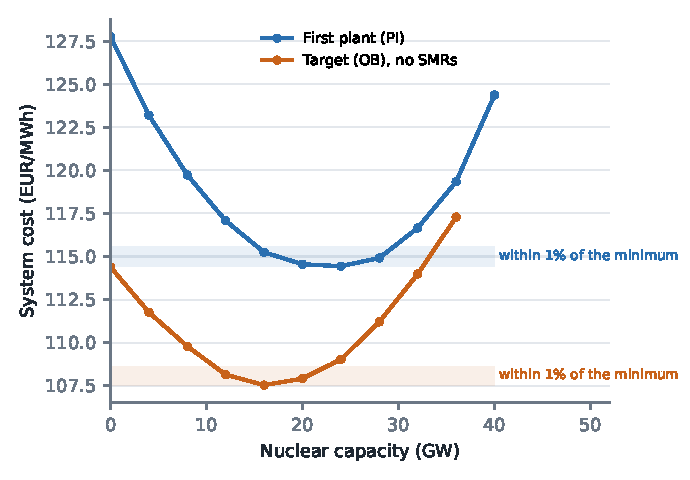
\includegraphics[width=0.52\linewidth]{fig_cost_en.pdf}
\caption{System cost against nuclear capacity at the central nuclear cost (fixN 911) and a 5\% cost of capital, three-hour step, with the band within 1\% of the minimum. Source: \texttt{results/v8\_runs.jsonl}.}\label{fig:cost}
\end{figure}

\subsection{Systems with and without nuclear}\label{sec:systems}
Table~\ref{tab:systems} compares the central systems at 5\%. In PI the system without nuclear needs 193\,GW of PV against 76, with every ground-mounted and agrivoltaic block at its cap, and two of the three industrial-roof blocks, and 59.6\,GW of onshore wind against 33.4, every block except the worst (10\,GW at 1{,}200 hours; 69.6\,GW are available). It needs 281\,GWh of batteries against 129 and 14.8\,TWh of hydrogen storage against 2.1, and it swaps 27.7\,TWh a year with the neighbours in each direction against 17.7. In cost terms, without nuclear PV costs 56.19\,EUR/MWh against 16.97, batteries 17.00 against 7.77 and hydrogen 11.22 against 4.98, and the system pays 4.57\,EUR/MWh of second grid charge above the 137\,GW threshold; the system with nuclear pays 65.43\,EUR/MWh for nuclear, which runs at a load factor of 87.5\%. In OB the system with nuclear relies on 10\,GW of CSP, 214\,GWh of compressed air and 310\,GWh of 100-hour storage next to 15.7\,GW of nuclear; without nuclear it adds PV (161\,GW against 85), batteries, hydrogen storage and 100-hour storage (632\,GWh). CSP is at its ceiling of 10\,GW in both OB systems; the ceiling is our assumption.

\begin{table}[!tb]
\centering\footnotesize
\caption{Central systems at 5\%, three-hour step. PV and onshore wind include the existing plants kept in the model. Hydrogen store in TWh (our conversion from GWh). Swap: energy exchanged with neighbours in each direction.}\label{tab:systems}
\begin{adjustbox}{max width=\linewidth}
\begin{tabular}{@{}lrrrrrrrrrrrr@{}}
\toprule
System & PV & Onshore & Offshore & Nuclear & CSP & Batteries & Hydrogen & Compr. & 100-hour & Intercon- & Swap & Nuclear\\
 & & wind & wind & & & & store & air & storage & nection & & load factor\\
 & GW & GW & GW & GW & GW & GWh & TWh & GWh & GWh & GW & TWh/yr & \%\\
\midrule
PI with nuclear & 76 & 33.4 & 0.0 & 23.2 & 0.0 & 129 & 2.1 & 0 & off & 13.9 & 17.7 & 87.5\\
PI without & 193 & 59.6 & 2.6 & 0.0 & 0.0 & 281 & 14.8 & 0 & off & 18.9 & 27.7 & \\
OB with nuclear & 85 & 44.6 & 0.0 & 15.7 & 10.0 & 13 & 4.1 & 214 & 310 & 13.6 & 20.2 & 89.1\\
OB without & 161 & 59.6 & 2.0 & 0.0 & 10.0 & 152 & 8.7 & 80 & 632 & 18.1 & 29.8 & \\
\bottomrule
\end{tabular}
\end{adjustbox}
\end{table}

\subsection{Variants}\label{sec:variants}
Table~\ref{tab:variants} gives the free optimum at 5\% when assumptions change. Nine rows change one assumption (the MACSE battery row changes the product, so price and duration together); two rows, marked as bundles, change several at once.

\emph{Trade.} If exports earn nothing the optimum is 25.4\,GW in PI and 18.3\,GW in OB; if they earn the import price it is 18.0 and 14.1\,GW. Allowing net exports changes little. Allowing net imports of up to 10\% of demand leaves the PI optimum at 23.4\,GW and lowers the OB optimum to 12.6\,GW. Choosing the critical weeks by low PV and wind output, as in the previous version, gives 18.2 and 14.5\,GW.

The trade rule of the previous version gives 11.9\,GW in PI and 7.2\,GW in OB, about half the central values, but it is a bundle of five changes: 38\% of the import capacity is available and counts as firm in the critical weeks; those weeks are chosen by low PV and wind output; imports cost 1.17 times the price in those weeks; nothing is exported; and there is no annual balance. Under it the model builds all 7.33\,GW of new lines and Italy imports 52 to 71\,TWh a year net. Taken one at a time: 10\% net imports give 23.4 and 12.6\,GW; weeks chosen by low PV and wind 18.2 and 14.5\,GW; the 38\% foreign credit alone, with the annual balance kept, 17.9 and 14.1\,GW. The credit is the largest single change in PI, about half of the drop, but only 1.6\,GW in OB. No single change explains the halving, which comes from the combination with the missing annual balance (Section~\ref{sec:dependence}).

\emph{Costs and weather.} With batteries at the MACSE award price (about 95\,EUR/kWh for systems of about 6.6 hours, against our 168.6 for 4-hour systems; not the same product), which also sets their duration at 6.6 hours, the optimum is 18.1 and 14.0\,GW: it stays at or above about 15\,GW in PI and near it in OB, so the recommendation of about 15\,GW does not change. Batteries move energy by hours, from day to evening, and that is already cheap; what nuclear replaces is firm energy in the winter weeks with little sun and wind, which without nuclear comes from hydrogen. Hydrogen, not batteries, is the bottleneck, and it is costed optimistically (Table~\ref{tab:limits}). With eight weather years, the four central ones and the four worst, it is 27.1\,GW in PI and 15.5\,GW in OB (about unchanged from 15.7); the added years reuse the load of 2016--2019, so there load and weather are not of the same year. A 7-year build gives 26.7 and 18.2\,GW. With nuclear at the top of the Commission bracket the optimum is 14.0\,GW in PI and 14.4\,GW in OB: OB has more nuclear than PI here, because its SMRs are at target cost and all 14.4\,GW are SMRs; with large reactors alone OB has 8\,GW (Table~\ref{tab:casesres}). The last row is the second bundle: the nuclear inputs of the previous version (8{,}540\,EUR/kW, 7 years, 80-year life, O\&M of 32\,EUR/MWh, availability 92\%; fixN 670) with the present costs of the other technologies.

With the annual balance and no foreign capacity in the critical weeks, the optimum is between 14.0 and 27.1\,GW in PI and between 14.0 and 18.3\,GW in OB in every variant except the bundle with the previous nuclear inputs (33.6 and 28.4\,GW). The variants that drop these rules give less: 12.6\,GW in OB with net imports up to 10\%, and 11.9 and 7.2\,GW with the trade rule of the previous version. Among the system rules the trade rule moves the result most; the cost of nuclear moves it more, since the cost cases span 0 to 40\,GW.

\begin{table}[!tb]
\centering\footnotesize
\caption{Variants at 5\%, free optimum, three-hour step. Each row changes one assumption, except the two bundles, which change several; the MACSE battery row changes the product, so price and duration together. Nuclear in GW (SMRs included); cost of the system with nuclear and saving against the system without nuclear under the same assumptions, EUR/MWh.}\label{tab:variants}
\begin{tabular}{@{}P{7.0cm}rrrrrr@{}}
\toprule
 & \multicolumn{3}{c}{PI} & \multicolumn{3}{c}{OB}\\
\cmidrule(lr){2-4}\cmidrule(l){5-7}
Variant & Nuclear & Cost & Saving & Nuclear & Cost & Saving\\
\midrule
Central & 23.2 & 114.42 & 13.35 & 15.7 & 107.53 & 6.86\\
Exports earn nothing & 25.4 & 117.20 & 15.26 & 18.3 & 110.50 & 8.58\\
Exports earn the import price (115.94\,EUR/MWh) & 18.0 & 111.10 & 11.86 & 14.1 & 103.71 & 5.56\\
Net imports allowed up to 10\% of demand & 23.4 & 114.11 & 11.81 & 12.6 & 107.12 & 4.09\\
Net exports allowed & 22.8 & 114.09 & 13.68 & 15.8 & 107.52 & 6.87\\
Critical weeks chosen by low PV and wind output & 18.2 & 113.64 & 10.45 & 14.5 & 107.03 & 6.50\\
Bundle: trade rule of the previous version (five changes, see text) & 11.9 & 109.99 & 5.96 & 7.2 & 103.38 & 2.14\\
Batteries at the MACSE award price, 6.6 hours & 18.1 & 108.92 & 11.38 & 14.0 & 105.09 & 4.99\\
Eight weather years (2016--2019, 1994, 1998, 2014, 2015) & 27.1 & 118.62 & 17.49 & 15.5 & 110.71 & 7.97\\
Nuclear built in 7 years & 26.7 & 112.02 & 15.75 & 18.2 & 105.90 & 8.48\\
Nuclear at the top of the Commission bracket (12{,}700\,EUR/kW) & 14.0 & 122.56 & 5.21 & 14.4$^{a}$ & 108.50 & 5.89\\
Bundle: nuclear inputs of the previous version (fixN 670) & 33.6 & 95.46 & 32.31 & 28.4 & 92.77 & 21.62\\
\bottomrule
\multicolumn{7}{@{}l}{$^{a}$ All SMRs at target cost.}
\end{tabular}
\end{table}

\subsection{Time step}\label{sec:step}
The same model at a six-hour step gives 21.7\,GW in PI and 13.7\,GW in OB at 5\%, against 23.2 and 15.7\,GW at three hours: the finer step raises the optimum by 1.6\,GW in PI (23.22 against 21.66) and 1.9\,GW in OB (15.65 against 13.73). The adequacy requirement is the same at both steps, so the difference does not come from the reserve. Hourly data were not rebuilt: the direction of the effect is known from the sequence of 12-, 6- and 3-hour steps (nuclear at 17.4, 21.7 and 23.2\,GW in PI and 6.0, 13.7 and 15.7\,GW in OB; the 12-hour runs are the repository's smoke tests, \texttt{tests/expected\_smoke\_h12.jsonl}), its size at one hour is not, so the three-hour results may still understate nuclear slightly. Only three-hour results are compared with each other in this paper.

\subsection{Small modular reactors in the target case}\label{sec:smr}
At their target cost SMRs are near-perfect substitutes of large reactors at the central cost: 934 against 911\,EUR/kW-yr at 5\%, and 1{,}231 against 1{,}239 at 7\%. The order changes with the rate because the 5-year build of SMRs, against 9 years, saves more interest during construction at 7\%; the 5 years is the vendor's schedule for the first Darlington unit, not an observed build, and with 7 years the advantage would disappear. The model therefore builds only large reactors at 5\% (15.7\,GW) and only SMRs at 7\% (11.1\,GW), but the choice is worth little: at 7\% the system with 11.0\,GW of large reactors and no SMRs costs 0.27\,EUR/MWh more (our calculation).

The OB curve with SMRs available (dotted in Fig.~\ref{fig:value}) shows the substitution. When large reactors are fixed below the optimum, SMRs fill the gap, so a further block of large reactors is worth only the cost of the SMRs it displaces: 934, 934 and 927\,EUR/kW-yr for the blocks between 4 and 16\,GW at 5\%, and 1{,}231 and 1{,}228 for the blocks between 4 and 12\,GW at 7\%. Its point at zero is the system with SMRs only (14.4\,GW at 5\%, 11.1\,GW at 7\%), which does not depend on the cost of large reactors, so the first block is also worth the SMRs it displaces (934 at 5\%, 1{,}231 at 7\%). The value of nuclear as a whole is the curve without SMRs; the two curves coincide from 16\,GW at 5\% and from 12\,GW at 7\%, where no SMR is built.

With SMRs at target cost, therefore, the system is almost insensitive to the cost of large reactors above about 934\,EUR/kW-yr. This rests on a target, the cost of the four-unit Darlington programme with the operating cost of large reactors as a proxy; at the first-plant cost (1{,}264\,EUR/kW-yr at 5\%) SMRs play no material role.
\FloatBarrier
